\documentclass[10pt,a4paper]{amsart}
\usepackage{amsmath,amssymb,amsthm,graphicx}
\usepackage[no-math]{fontspec}
\setmainfont{DejaVu Serif}
\setmonofont{DejaVu Sans Mono}
\usepackage{amsmath,amssymb,graphicx,xcolor,tikz-cd,verbatim}
\usetikzlibrary{calc,positioning,arrows.meta,quotes}
\usepackage{hyperref}
\usepackage[capitalise]{cleveref}
\newtheorem{theorem}{Theorem}
\newtheorem{proposition}[theorem]{Proposition}
\newtheorem{lemma}[theorem]{Lemma}
\theoremstyle{definition}
\newtheorem{definition}[theorem]{Definition}
\newtheorem{example}[theorem]{Example}
\newtheorem{remark}[theorem]{Remark}

% BEGIN unchanged author macros.sty
% General maths
\newcommand{\set}[1]{\{#1\}}
\newcommand{\Z}{\mathbb{Z}} % integers
\newcommand{\freegroup}[1]{#1^*} % free group
\newcommand{\freemonoid}[1]{#1^+} % free monoid
% \newcommand{\emptyword}{\varepsilon} % empty word
\newcommand{\id}{\operatorname{id}} % identity
\newcommand{\dom}{\operatorname{dom}} % domain
\newcommand{\code}{\texttt} % code
\newcommand{\into}{\hookrightarrow} % injective map
\newcommand{\pres}[2]{\langle #1\ |\ #2\rangle} % presentation
\newcommand{\monpres}[2]{\pres{#1}{#2}^+} % monoid presentation
% \newcommand{\pgroup}[1]{\overline{#1}} % presented group
\newcommand{\pgroup}[1]{[#1]} % presented group
\newcommand{\pmonoid}[1]{[#1]^+} % presented monoid
\newcommand{\sizeof}[1]{|#1|} % cardinal
\newcommand{\nf}{\widehat} % normal form

% HoTT
\let\S\undefined
\newcommand{\S}[1]{\operatorname{S}^{#1}} % sphere
\newcommand{\B}{\operatorname{B}} % delooping
\newcommand{\pt}[1]{\star_{#1}} % pointed element
\newcommand{\trunc}[2]{\|#2\|_{#1}} % truncation
\newcommand{\ptrunc}[1]{\trunc{-1}{#1}} % propositional truncation
\newcommand{\strunc}[1]{\trunc0{#1}} % set truncation
\newcommand{\gtrunc}[1]{\trunc1{#1}} % groupoid truncation
\newcommand{\trunq}[2]{|#2|_{#1}} % quotient map to the truncation
\newcommand{\ptrunq}[1]{\trunq{-1}{#1}} % quotient map to the propositional truncation
\newcommand{\strunq}[1]{\trunq0{#1}} % quotient map to the set truncation
\newcommand{\defd}{:=} % defined as
\newcommand{\qdefd}{\quad\defd\quad}
\newcommand{\ptorsor}[1]{\operatorname{P}_{#1}} % principal torsor
\newcommand{\K}{\operatorname{K}} % Eilenberg-Mac Lane
\newcommand{\EM}[2]{\K(#1,#2)} % K(G,n)
\newcommand{\Cayley}[2]{\operatorname{C}(#1,#2)}
\newcommand{\refl}[1]{\operatorname{refl}_{#1}} % constant path
\newcommand{\pcomp}{\cdot} % concatenation of paths
\newcommand{\sym}[1]{#1^-} % inverse
\newcommand{\J}{\operatorname{J}} % induction for paths
\newcommand{\equivto}{\simeq} % equivalence between types
\newcommand{\transport}[1]{#1^\to} % transport
\newcommand{\transportinv}[1]{#1^\ot} % transport in backward direction
\newcommand{\subst}[2]{#1^\to_{#2}} % substitution
\newcommand{\happly}[2]{#1(#2)} % apply an equality between functions
\newcommand{\Beq}[1]{\operatorname{d}_{#1}} % equality ΩBG = G
\newcommand{\End}{\operatorname{End}} % endomorphisms
\newcommand{\Aut}{\operatorname{Aut}} % automorphisms
\newcommand{\Fin}{\operatorname{Fin}} % finite type
\newcommand{\isContr}{\operatorname{isContr}} % contractible
% \newcommand{\isSurj}{\operatorname{isSurj}} % surjective
\newcommand{\hasSect}{\operatorname{hasSect}} % has a section
\newcommand{\Comp}{\operatorname{Comp}} % connected component
\newcommand{\Loop}{\operatorname{\Omega}} % loop space
\let\P\undefined
\newcommand{\P}[1]{\operatorname{P}_{#1}} % principal torsor
\let\cong\undefined
\newcommand{\cong}[1]{#1^=} % congruence
\newcommand{\ap}{\cong}
% \newcommand{\fst}{\operatorname{fst}} % first projection
% \newcommand{\snd}{\operatorname{snd}} % second projection
\newcommand{\fst}{\pi}
\newcommand{\snd}{\pi'}
\newcommand{\incl}{\iota} % canonical inclusion
\newcommand{\isSet}{\operatorname{isSet}} % being a set
\newcommand{\isGroupoid}{\operatorname{isGroupoid}} % being a groupoid
\newcommand{\underlying}[1]{\langle #1\rangle} % underlying something
\newcommand{\hq}{\mathop{\!/\!\!/\!}} % homotopy quotient
\newcommand{\fib}[1]{\operatorname{fib}_{#1}} % fiber
\newcommand{\toGroup}{\to_{\operatorname{Grp}}} % morphisms of group

% Types
\newcommand{\U}{\mathcal{U}} % the universe
\newcommand{\Type}{\U} % the universe
\newcommand{\Endomorphisms}{\Type^{\circlearrowleft}} % endomorphisms
\newcommand{\SetEnd}{\Set^{\circlearrowleft}} % endomorphisms of a set
\newcommand{\Prop}{\operatorname{Prop}} % the type of propositions
\newcommand{\Set}{\operatorname{Set}} % the type of sets
% \newcommand{\Groupoid}{\operatorname{Groupoid}} % the type of groupoids
\newcommand{\Group}{\operatorname{Group}} % the type of groups
\newcommand{\IGroup}[1][1]{\operatorname{IntGroup}} % the type of internal groups
\newcommand{\GSet}[1][G]{\Set_{#1}} % G-sets
\newcommand{\GSetEquiv}[3][G]{#2\simeq^{\GSet[#1]}#3} % equivalence between G-sets
\newcommand{\XSet}[1][X]{\Set_{#1}} % G-sets
\newcommand{\Torsors}{\operatorname{Tors}}
\newcommand{\GTors}[1][G]{\Torsors_{#1}} % G-torsors
\newcommand{\XTors}[1][X]{\Torsors_{#1}} % X-torsors

% Constructors
\newcommand{\constructor}[1]{\operatorname{\textsf{\textup{#1}}}}
\newcommand{\cloop}{\constructor{loop}}
\newcommand{\cloopcomp}{\constructor{loop-comp}}
\newcommand{\cloopid}{\constructor{loop-id}}
\newcommand{\ctrunc}{\constructor{trunc}}
\newcommand{\cgen}{\constructor{gen}}
\newcommand{\crel}{\constructor{rel}}
\newcommand{\cvertex}{\constructor{vertex}}
\newcommand{\cv}{\constructor{v}}
\newcommand{\cedge}{\constructor{edge}}
\newcommand{\ce}{\constructor{e}}
\newcommand{\ccell}{\constructor{cell}}
\newcommand{\cpath}{\constructor{path}}

% Groups
\newcommand{\gm}{m} % multiplication
\let\ge\undefined
\newcommand{\ge}{e} % unit
\newcommand{\gi}{i} % inverse
\newcommand{\inv}[1]{#1^{-1}}

% Shortcuts
\newcommand{\pa}[1]{\left(#1\right)}
\newcommand{\ol}{\overline}
\let\ul\undefined
\newcommand{\ul}{\underline}

% Symbols
\newcommand{\ot}{\leftarrow}
\newcommand{\To}{\Rightarrow}

% Spacing
\newcommand{\qeq}{\quad=\quad}

% English
\newcommand{\ie}{i.e.~}
\newcommand{\eg}{e.g.~}
\newcommand{\resp}{resp.~}
\newcommand{\aka}{aka~}
\newcommand{\wrt}{wrt~}

% Misc
\newcommand{\agda}[2]{\href{https://smimram.github.io/generated-deloopings-agda/#1.html\##2}{\texttt{#1.#2}}}
% \newcommand{\TODO}[1]{}
\newcommand{\TODO}[1]{\marginpar{\tiny #1}}
\newcommand{\SM}[1]{\TODO{SM: #1}}
\newcommand{\EO}[1]{\TODO{EO: #1}}
% \newcommand{\CC}[1]{\TODO{CC: #1}}
\newcommand{\AR}[1]{\TODO{AR: #1}} % anonymous reviewer

% Local Variables:
% TeX-master: "article"
% End:

% END unchanged author macros.sty
\title{The Cayley graph is the homotopy fiber of the delooped generating map}
\author{Camil Champin, Samuel Mimram, Émile Oleon}
\date{doi:10.4230/LIPIcs.FSCD.2024.6; CC BY4.0 (fixed arXivv1 author source)}
\begin{document}
\maketitle
\setcounter{section}{1}
\noindent\textit{Editorial note.} Source https://drops.dagstuhl.de/entities/document/10.4230/LIPIcs.FSCD.2024.6 and author-linked https://arxiv.org/abs/2405.03264v1 . The fixed author full version is itself CC BY4.0; native mathematical text, figures and complete omitted-proof appendix retained.\par\medskip
\noindent\textit{Allowed standard prerequisites (editorial).}\begin{itemize}
\item Homotopy type theory with univalence, higher inductive types, groupoid truncation and free-group universal properties. Author hott.tex and complete source-local constructions/proof appendix retained; standard results are cited to the HoTT Book. No independent Agda execution or correctness certification is performed.
\end{itemize}\medskip
\section{Homotopy type theory}
\label{hott}
We unfortunately do not have enough space here to provide an introduction from
scratch to dependent type theory and homotopy type theory, so we refer the reader
to the reference book for an in depth presentation~\cite{hottbook}. The main
purpose of this section is to fix some terminology and notations for classical
notions.

\paragraph{Universe}
We write $\U$ for the \emph{universe}, \ie the large type of all small types,
which we suppose to be closed under dependent sums and products. We write
$\Pi(x:A).B$ or $(x:A)\to B$ for $\Pi$-types, and $A\to B$ for the case
where~$B$ is non-dependent. Similarly, we write $\Sigma(x:A).B$ for
$\Sigma$-types, and $A\times B$ for the non-dependent version. The two
projections from a $\Sigma$-type are respectively written $\fst$ and $\snd$.

\paragraph{Paths}
Given a type $A:\U$ and two elements $a,b:A$, we write $a=_A b$ for the type of
\emph{identities}, or \emph{paths}, between~$a$ and~$b$: its elements are proofs
of equality between $a$ and $b$. In particular, for any $a:A$, the type $a=a$
contains the term $\refl{a}$ witnessing for reflexivity of
equality.
%
We sometimes write $x\defd t$ to indicate that $x$ and $t$ are equal by
definition.
%
The elimination principle of identities, \aka \emph{path induction} and often
noted~$J$, roughly states that, given $a:A$, in order to show a property
$P:(x:A)\to(a=x)\to\U$ for every $x:A$ and $p:a=x$ it is enough to show it in
the case where $x\defd a$ and $p\defd\refl{a}$.
%
% Given a $a:A$ and a property $P:(x:A)\to(a=x)\to\U$, the canonical map
% \begin{align*}
  % \pa{(x:A)\to(p:a=x)\to P\,x\,p}&\to P\,a\,\refl{a}
  % % f&\mapsto f\,\,\refl{a}
% \end{align*}
% given by evaluation at $\refl{a}$ is an equivalence. In particular, it admits
% an inverse, which encodes the induction principle for paths (\aka \emph{path
% induction}) and is commonly noted~$\J$: in order to show a property~$P$
% depending on a path~$p$ whose target endpoint is free, it is enough to show it
% when the path is $\refl{}$.
%
By path induction, the following can be shown. Given a type~$A$ and a type
family $B:A\to\U$, a path $p:x=y$ in~$A$ induces a function
$\subst Bp:B(x)\to B(y)$ witnessing for the fact that equality is
\emph{substitutive}. As a special case, any path $p:A=B$ between two
types~$A,B:\U$ induces a function $\transport p:A\to B$, called the
\emph{transport} along~$p$, as well as an inverse function
$\transportinv p:B\to A$. Finally, given a function $f:A\to B$, any path $p:x=y$
in~$A$ induces a path $\cong f(p): f(x) = f(y)$ witnessing for the fact that
equality is a \emph{congruence}.

\paragraph{Higher inductive types}
Many functional programming languages allow the definition of inductive types,
which are freely generated by constructors. For instance, the type~$\S0$ of
booleans is generated by two elements (true and false).
%
In the context of homotopy type theory, languages such as cubical Agda feature a
useful generalization of such types, called \emph{higher inductive types}. They allow, in addition to traditional constructors for elements of the type,
constructors for equalities between elements of the type. For instance, the type
corresponding to the circle $\S1$ can be defined as generated by two points $a$
and $b$ and two equalities $p,q:a=b$ between those points.
% \begin{center}
% \begin{minipage}{0.4\linewidth}
% \begin{verbatim}
% data S¹ : Type where
  % a b : S¹
  % p q : a ≡ b
% \end{verbatim}
% \end{minipage}
% \begin{minipage}{0.4\linewidth}
  % \[
    % \begin{tikzpicture}[baseline=(current bounding box.center)]
      % \filldraw (-.5,0) circle (0.05) node[left] {$a$};
      % \filldraw (.5,0) circle (0.05) node[right] {$b$};
      % \draw (0,0) circle (.5);
      % \draw (0,.5) node[below]{$p$};
      % \draw (0,-.5) node[above]{$q$};
    % \end{tikzpicture}
  % \]
% \end{minipage}
% \end{center}
Higher-dimensional spheres~$\S n$ can be defined in a similar way.

\paragraph{Univalence}
\label{equivalence}
A map $f:A\to B$ is an \emph{equivalence} when it admits both a left and a right
inverse. In particular, every isomorphism is an equivalence. We write
$A\equivto B$ for the type of equivalences from~$A$ to~$B$. The identity is
clearly an equivalence and we thus have, by path induction, a canonical map
$(A=B)\to(A\equivto B)$ for every types~$A$ and~$B$: the \emph{univalence axiom}
states that this map is itself an equivalence.
%
In particular, every equivalence $A\equivto B$ induces a path $A=B$.
%
It is known that univalence implies the \emph{function extensionality}
principle~\cite[Section~2.9]{hottbook}: given functions $f,g:A\to B$, if
$f(x)=g(x)$ for any $x:A$ then $f=g$ (and the expected generalization to
dependent function types is also valid).

\paragraph{Homotopy levels}
A type~$A$ is \emph{contractible} when the type $\Sigma(x:A).(y:A)\to(x=y)$ is
inhabited: this means that we have a ``contraction point'' $a_0 : A$, and a
continuous family of paths from $a_0$ to every other point in $A$.
%
A type~$A$ is a \emph{proposition} (\resp a \emph{set}, \resp a
\emph{groupoid}) when $(x=y)$ is contractible (\resp a proposition, \resp a
set) for every $x,y:A$. Intuitively, a contractible type is a point (up to
homotopy), a proposition is a point or is empty, a set is a collection of points
and a groupoid is a space which bears no non-trivial 2-dimensional (or higher)
structure.
% For instance, consider the following three types corresponding to
% spheres of respective dimensions $-1$, $0$, $1$ and $2$:
% \AR{Usually (eg in [HoTT Book, §6.5]) the $-1$-sphere is taken to be the empty
% type, not the contractible type, so that $\Sigma\S{-1}\equivto\S0$.}
% \[
  % \begin{array}{c@{\qquad\qquad\qquad}c@{\qquad\qquad\qquad}c@{\qquad\qquad\qquad}c}
    % % \begin{tikzpicture}
      % % \filldraw (0,0) circle (.05);
      % % \draw (0,-.5);
    % % \end{tikzpicture}
    % &
    % \begin{tikzpicture}
      % \filldraw (0,0) circle (.05);
      % \filldraw (1,0) circle (.05);
      % \draw (.5,-.5);
    % \end{tikzpicture}
    % &
    % \begin{tikzpicture}
      % \filldraw (0,0) circle (.05);
      % \filldraw (1,0) circle (.05);
      % \draw (.5,0) circle (.5);
    % \end{tikzpicture}
    % &
    % % https://tex.stackexchange.com/questions/348609/draw-a-3d-sphere-with-radius-with-tikz
    % \begin{tikzpicture}
      % \shade[ball color = gray!40, opacity = 0.4] (.5,0) circle (.5);
      % \draw (.5,0) circle (.5);
      % \draw (0,0) arc (180:360:.5 and 0.2);
      % \draw[dotted] (1,0) arc (0:180:.5 and 0.2);
      % \filldraw (0,0) circle (.05);
      % \filldraw (1,0) circle (.05);
    % \end{tikzpicture}
    % \\
    % \S{-1}&\S0&\S1&\S2
  % \end{array}
  % \]
% For instance, the sphere $\S{-1}$ (\ie the empty type) is a proposition, the
% sphere $\S0$ (\ie the booleans) is a set and the sphere $\S1$ (\ie the circle)
% is a groupoid, and the sphere $\S2$ is not a groupoid (because there is a
% 2-dimensional ``hole'' in it).
%
We write $\Set$ for the type of sets. Given a type~$A$, we write $\isSet(A)$ (\resp $\isGroupoid(A)$) for the predicate indicating that~$A$ is a set (\resp groupoid).

\paragraph{Truncation}
Given a type $A$, its \emph{propositional truncation} turns it into a
proposition in a universal way. It consists of a type~$\ptrunc{A}$, which is a
proposition, equipped with a map~$\ptrunq-:A\to\ptrunc{A}$ such that, for any
proposition~$B$, the map $(\ptrunc A\to B)\to(A\to B)$ induced by precomposition
by~$\ptrunq-$ is an equivalence. Intuitively, the type $\ptrunc A$ behaves like~$A$,
except that we do not have access to its individual elements: the elimination
principle for propositional truncation states that in order to construct an
element of~$B$ from an element of~$\ptrunc A$, we can only assume that we have
an element of~$A$ if~$B$ itself is a proposition.
%
The \emph{set truncation} $\strunc A$ of a type~$A$ is defined similarly, as the
universal way of turning~$A$ into a set, and we write $\strunq{x}$ for the image
of~$x:A$ in the truncation; and we can similarly define the \emph{groupoid truncation}~$\gtrunc A$.

\paragraph{Fibers}
Given a function $f:A\to B$, we write $\fib fb$ for the type $\Sigma(a:A).(f\,a=b)$, called the \emph{fiber} of~$f$ at $b$. The function $f$ is said to be \emph{surjective} when the type $(b:B)\to\ptrunc{\fib fb}$ is inhabited, \ie when every element of $B$ merely admits a preimage.


% Local Variables:
% TeX-master: "article"
% End:

\section{Delooping groups}
\label{delooping}

\paragraph{The external point of view}
A \emph{group} consists of a set $A$, together with an operation
$\gm:A\to A\to A$ (the \emph{multiplication}), an element $\ge:A$ (the
\emph{unit}), and an operation $\gi:A\to A$ (the \emph{inverse}) such that
multiplication is associative, admits $\ge$ as unit, and $\gi(x)$ is the
two-sided inverse of any element $x:A$. We write $\Group$ for the type of all
groups, and $G\toGroup H$ for the type of group morphisms between groups~$G$
and~$H$.
% :
% \begin{align*}
  % \Group\defd
  % \Sigma(A:\Set).&
  % (\gm:A\to A\to A)\times(\ge:A)\times(\gi:A\to A)\times
  % \\
  % &((x,y,z:A)\to\gm(\gm(x,y),z)=\gm(x,\gm(y,z))\times
  % \\
  % &((x:A)\to\gm(\ge,x)=\gm(x,\ge)=x)\times
  % \\
  % &((x:A)\to\gm(\gi(x),x)=\gm(x,\gi(x))=e)
% \end{align*}
%
In the following, we use the traditional notations for groups: given two
elements $x,y:G$, we simply write $xy$ instead of $\gm(x,y)$, $1$ instead of
$\ge$, and $x^{-1}$ instead of $\gi(x)$.

\paragraph{The internal point of view}
\label{internal-groups} 
A \emph{pointed} type consists of a type~$A$ together with a distinguished
element, often written~$\pt{}$ and sometimes left implicit. Given a pointed type
$(A,\pt{})$, its \emph{loop space}~$\Loop A$ is defined as the type of paths
from $\pt{}$ to itself: $\Loop A\defd(\pt{}=\pt{})$. The elements of this type
are called \emph{loops}. By path induction one can construct, for every two
paths $p:a=b$ and $q:b=c$, a path in $a=c$ called their \emph{concatenation} and
written $p\pcomp q$. Similarly, every path~$p:a=b$, admits an \emph{inverse}
path $\sym p:b=a$. When~$A$ is a pointed groupoid, $\Loop A$ is a set, and these
operations canonically equip this set with a structure of
group~\cite[Section~2.1]{hottbook}.

\paragraph{Delooping groups}
A \emph{delooping} of a group~$G$ is a pointed connected groupoid $\B G$
together with an identification $\Beq G:\Loop\B G=G$ (we recall that a type~$A$
is \emph{connected} when the type~$\strunc{A}$ is contractible, \ie $A$ has one
connected component).
%
The notation is justified by the fact that deloopings are unique.
%
For instance, it is known that the circle is a delooping of~$\Z$: indeed, $\S1$ is a connected groupoid, and its fundamental group is~$\Z$~\cite[Section~8.1]{hottbook}.

% Local Variables:
% TeX-master: "article"
% End:

\section{Delooping using higher inductive types}
\label{delooping-hit}

\paragraph{Delooping as a higher inductive type}
Given a group~$G$, its delooping should have a point~$\pt{}$ and a loop for
every element of the group. Moreover, we should ensure that the multiplication
of $G$ coincides with the concatenation operation on the loop space, and that
the type we obtain is a (pointed connected) groupoid. This suggests considering
a higher inductive type, noted $\K(G,1)$, with the following constructors
\[
  \begin{array}{l@{\ :\ }l}
    \pt{}&{\K(G,1)}\\
    \cloop&G\to\pt{}=\pt{}\\
    \cloopcomp&(x,y:G)\to\cloop x\pcomp\cloop y=\cloop(xy)\\
    % \cloopid&\cloop 1=\refl{}\\
    \ctrunc&\isGroupoid(\K(G,1))
  \end{array}
\]
This construction was first proposed by Finster and Licata. They also showed,
using the encode-decode method, that it is a delooping of the original group,
\ie $\Loop\K(G,1)=G$, see~\cite[Theorem~3.2]{licata2014eilenberg}. Note that we
only ask here that $\cloop$ preserves multiplication (with $\cloopcomp$),
because it can be shown that this implies preservation of unit and inverses. In
particular, preservation of unit (see \agda{EM}{loop-id}) renders superfluous
one of the constructors present in the original
definition~\cite{licata2014eilenberg}.

In the following, we will define a variant of this higher inductive type when
the group~$G$ is presented, which is smaller and gives rise to computations
closer to traditional group theory.

\paragraph{Presentations of groups}
Given a set~$X$, we write $\freegroup{X}$ for the \emph{free group}
over~$X$~\cite[Theorem~6.11.6]{hottbook}. There is an inclusion
function~$\incl:X\to\freegroup{X}$ which, by precomposition, induces an
equivalence between morphisms of groups~$\freegroup{X}\to G$ and
functions~$X\to G$. We write $\freegroup{f}:\freegroup{X}\to G$ for the group
morphism thus induced by a function~$f:X\to G$.
% This group is such that, for any group~$G$, a function $X\to G$ extends
% uniquely as a group morphism~$\freegroup{X}\to G$.
The elements of~$\freegroup X$ can be described as formal
composites~$a_1\ldots a_n$ where each $a_i$ is an element of~$X$ or a formal
inverse of an element of~$X$ (such that an element with an adjacent formal
inverse cancel out).

Any free group~$\freegroup X$ admits a delooping as a wedge of an $X$-indexed familly of circles. The corresponding type~$\bigvee_X\S1$ can be described as the coequalizer
\begin{equation}
  \label{wedge-of-circles}
  \begin{tikzcd}
    X\ar[r,shift left]\ar[r,shift right]&1\ar[r,dotted]&\bigvee_X\S1
  \end{tikzcd}
\end{equation}
or, equivalently, as the higher inductive type
% \[
  % \begin{array}{l@{\ :\ }l}
    % \pt{}&\bigvee_X\S1\\
    % \cloop&X\to\pt{}=\pt{}
  % \end{array}
  % \]
generated by the two constructors $\pt{}:\bigvee_X\S1$ and $\cloop:X\to\pt{}=\pt{}$.

\begin{proposition}
  \label{bouquet-loop-space}
  We have $\Loop\bigvee_X\S1=\freegroup{X}$, \ie the above type is a $\B\freegroup X$.
\end{proposition}
\begin{proof}
  The fact that $\bigvee_X\S1$ is a delooping of~$\freegroup X$ is not too difficult to show when~$X$
  has decidable equality, see~\cite[Exercise 8.2]{hottbook}
  and~\cite{kraus2018free}, but the general case is more involved and was recently proved
  in~\cite{warn2023path}: the main issue is to show that this type is a groupoid.
\end{proof}

A group \emph{presentation} $\pres XR$ consists of a set~$X$ of
\emph{generators}, a set~$R$ of \emph{relations}, and two functions
$\fst,\snd:R\to\freegroup X$ respectively associating to a relation its
\emph{source} and \emph{target}. We often write $r:u\To v$ for a
relation~$r$ with $u$ as source and~$v$ as target.
%
Given such a presentation~$P$, the corresponding \emph{presented} group~$\pgroup P$ is the set quotient $\freegroup{X}/R$ of the free group on $X$ under the
smallest congruence identifying the source and the target of every
relation~$r:R$. This type can be described as the type
$\pgroup P\defd\strunc{{\freegroup X}\hq R}$ obtained by taking the set
truncation of the coequalizer
\[
  \begin{tikzcd}
    R
    \ar[r,shift left,"\fst"]
    \ar[r,shift right,"\snd"']
    &
    \freegroup X
    \ar[r,dotted,"\kappa"]
    &
    \freegroup X\hq R
  \end{tikzcd}
\]
From this also follows a description of~$\pgroup P$ as a higher inductive type:
\[
  \begin{array}{l@{\ :\ }l}
    \constructor{word}&\freegroup X\to\pgroup P\\
    \constructor{rel}&(r:R)\to\constructor{word}(\fst(r))=\constructor{word}(\snd(r))\\
    \ctrunc&\isSet(\pgroup P)
  \end{array}
\]

\paragraph{A smaller delooping}
Suppose given a group~$G$ along with a presentation $P\defd\pres XR$, \ie such that $G=\pgroup P$. We define the type $\B P$ as the following higher inductive type:
\[
  \begin{array}{l@{\ :\ }l}
    \pt{}&{\B P}\\
    \cgen&X\to(\pt{}=\pt{})\\
    \crel&(r:R)\to(\freegroup\cgen(\fst(r))=\freegroup\cgen(\snd(r)))\\
    \ctrunc&\isGroupoid(\B P)
  \end{array}
\]
This type is generated by a point~$\pt{}$, then the constructor~$\cgen$ adds a
loop~$\ul a:\pt{}=\pt{}$ for every generator~$a$, the constructor~$\crel$ adds
an equality
$\ul a_1\pcomp\ul a_2\pcomp\ldots\pcomp\ul a_n=\ul b_1\pcomp\ul
b_2\pcomp\ldots\pcomp\ul b_m$ for each relation
$a_1\ldots a_n\To b_1\ldots b_m$, and the constructor~$\ctrunc$ formally takes
the groupoid truncation of the resulting type. Note that, because of the
presence of $\freegroup\cgen:\freegroup X\to(\pt{}=\pt{})$ in the type
of~$\crel$, the above inductive type is not accepted as is in standard proof
assistants such as Agda. However, a definition can be done in two stages, by
first considering $\bigvee_X\S1$ (\ie the type generated only by $\pt{}$ and $\cgen$), and then defining a
second inductive type further quotienting this type (\ie adding the
constructors $\crel$ and $\ctrunc$), see \agda{EM}{Delooping}. Also, the
definition of $\freegroup\cgen$ requires the group structure on $\bigvee_X\S1$: the group operations are easily defined from operations on paths (reflexivity, concatenation, symmetry), but the fact that it is a groupoid is non-trivial (see \cref{bouquet-loop-space}).
%
Our main result in this section is the following:

\begin{theorem}[\agda{EM}{theorem}]
  \label{presented-delooping}
  Given a presentation~$P\defd\pres XR$, the type $\B P$ is a delooping of the group~$\pgroup P$.
\end{theorem}
\begin{proof}
  % agda -> latex
  % loop -> g'
  % path -> gen*
  %
  By induction on~$\B P$, we can define a function $f:\B P\to\K(\pgroup P,1)$ such that
  $f\pt{}\defd\pt{}$, and $f(\cgen a)\defd\cloop\pgroup a$ for all $a:X$. It can
  be shown that $f$ is then such that
  $\cong f(\freegroup\cgen u)=\cloop\pgroup u$, for any $u:\freegroup X$. We can
  therefore define the image $\cong f(r)$ on a relation $r:u\To v$ as the
  composite of equalities
  \[
    \cong f(\freegroup\cgen u)=\cloop\pgroup u=\cloop\pgroup v=\cong f(\freegroup\cgen v)
  \]
  where the equality in the middle follows from the fact that we have
  $\pgroup u=\pgroup v$ because of the relation~$r$.

  In the other direction, the group morphism $\freegroup\cgen:\freegroup{X}\to \Loop\B P$ preserves relations (by~$\crel$), and thus induces a quotient morphism $g':\pgroup P\to\Loop\B P$.
  We can thus consider the function $g:\K(\pgroup P,1)\to\B P$ such that $g(\pt{})=\pt{}$, for $x:\pgroup P$ we have $\ap g(\cloop x)=g'(x)$, and for $x,y:\pgroup P$ the image of $\cloopcomp x\,y$ is canonically induced by the fact that $g'$ preserves group multiplication.

  Since $\K(\pgroup P,1)$ is a groupoid, in order to show that $f(g(x))=x$ for every $x:\K(\pgroup P,1)$, it is enough to show that it holds for $x\defd\pt{}$, which is the case by definition of $f$ and $g$, and that this property is preserved under $\cloop x$ for $x:\pgroup P$, which follows from the fact that we have $\ap f(g'(x))=\cloop x$ for any~$x:\pgroup P$ (this is easily shown by induction on~$x$).
  %
  Conversely, we have to show that $g(f(x))=x$ holds for $x:\B P$. Again, this is shown by induction on~$x$.
  %
  % \TODO{terminer ceci}
  %
  % $\sigma$ is a section of $\strunq-\circ\kappa:\freegroup X\to\pgroup P$, and
  % the fact that $g(f(x))=x$ for $x:\B P$ follows from the fact that $\sigma$
  % preserves generators.
\end{proof}

\noindent
As an interesting remark, the careful reader will note that the fact that the types $X$ and $R$ are sets does not play a role in the proof: in fact, those assumptions can be dropped here.
%
Also, note that we do not need the choice of a representative in $\freegroup X$ for every element of $\pgroup P$ in order to define the function $g$ from $\freegroup\cgen$ in the above proof: intuitively, this is because the induced function~$g$ does not depend on such a choice of representatives.
%
Finally, we should mention here that a similar result is mentioned as an exercise in \cite[Example 8.7.17]{hottbook}; the proof suggested there is more involved since it is based on a generalized van Kampen theorem.

\begin{example}
  The dihedral group $D_5$, see \cref{Dn}, admits the presentation
  \[
    \pres{r,s}{r^4=srs,sr^2s=r^3,rsr=s,r^3s=sr^2,sr^3=r^2s,s^2=1}
  \]
  Hence, by \cref{presented-delooping} we can construct a delooping of $D_5$ as an
  higher inductive type generated by two loops (corresponding to~$r$ and $s$)
  and six $2$-dimensional cells (corresponding to the relations). Note that this
  is much smaller than $\K(D_5,1)$ (it has 2 instead of 10 generating loops, and
  6 instead of 100 relations), thus resulting in shorter proofs when reasoning
  by induction.
\end{example}

\begin{example}
  Any group~$G$ admits a presentation, the \emph{standard presentation}, with one generator $\ul a$ for every element $a:G$, and relations $\ul a\,\,\ul b=\ul{ab}$ for every pair of generators, as well as $\ul 1=1$. By applying \cref{presented-delooping}, we actually recover the inductive type~$\K(G,1)$ as delooping of~$G$.
\end{example}

% Local Variables:
% TeX-master: "article"
% End:

\section{Delooping with torsors}
\label{torsor-delooping}
In this section, we recall the other classical approach to constructing
deloopings of groups by using $G$-torsors, which originates in classical
constructions of algebraic topology~\cite{demazure1970groupes}. Most of the
material of the section is already known, for which reason proofs are not much
detailed. A more in-depth presentation can be found in recent works such
as~\cite{symmetry,buchholtz2023central}.

\paragraph{Group actions}
% \label{group-action}
Given a group~$G$ and a set~$A$, an \emph{action} of $G$ on $A$ is a group
morphism from $G$ to $A \simeq A$, that is a map $\alpha : G\to (A \simeq A)$
such that
\begin{align}
  \label{action-equations}
  \alpha(xy)&= \alpha(x) \circ \alpha(y)
  &
  \alpha(1) &= \id_A
\end{align}
% $\alpha(xy)= \alpha(x) \circ \alpha(y)$
% and
% $\alpha(1) = \id_A$
for all $x,y:G$.

A \emph{$G$-set} is a set equipped with an action of~$G$, and we write $\GSet$
for the type of $G$-sets. We often simply denote a $G$-set by the associated
action $\alpha$ and write $\dom(\alpha)$ for the set on which~$G$ acts.

\begin{lemma}[\agda{GSetProperties}{isGroupoidGSet}]
  \label{gset-groupoid}
  The type $\GSet$ is a groupoid.
\end{lemma}
\begin{proof}
  The type of sets is a groupoid~\cite[Theorem 7.1.11]{hottbook}. Given a set
  $A$, the type of functions $A\to A$ is a set~\cite[Theorem 7.1.9]{hottbook}
  and thus a groupoid. Finally,
  % the equations \cref{action-equations}
  the axioms~\cref{action-equations} of actions are propositions (because $A$
  is a set) and thus groupoids. We conclude since groupoids are closed under
  $\Sigma$-types~\cite[Theorem 7.1.8]{hottbook}.
\end{proof}

Given $G$-sets $\alpha$ and $\beta$, a \emph{morphism} between them consists of
a function $f:\dom{\alpha}\to \dom{\beta}$ which preserves the group action, in
the sense that for every $x:G$ and $a:\dom{\alpha}$, we have
\begin{equation}
  \label{G-set-morphism}
  \beta(x)(f(a))=f(\alpha(x)(a))
  \text.
\end{equation}
A morphism which is also an equivalence is called an \emph{isomorphism} and we
write $\GSetEquiv\alpha\beta$ for the type of isomorphisms between $\alpha$ and
$\beta$. We write $\Aut(\alpha)$ for the type of automorphisms
$\GSetEquiv\alpha\alpha$, which is a group under composition.
%
% \subsubsection{Identities of~$G$-sets}
The equalities between $G$-sets can be conveniently characterized as follows.

\begin{proposition}[\agda{GSetProperties}{GSet≡Decomp}]
  \label{Gset-equalities}
  Given two $G$-sets $\alpha$ and $\beta$, an equality between them consists of
  an equality $p:\dom{\alpha}=\dom{\beta}$ such that the function induced by
  transport along~$p$, namely $\transport p:\dom\alpha\to\dom\beta$, is a
  morphism of $G$-sets.
\end{proposition}
\begin{proof}
  The characterization of equalities between
  $\Sigma$-types~\cite[Theorem~2.7.2]{hottbook} entails that an equality between
  $(\dom{\alpha},\alpha)$ and $(\dom{\beta},\beta)$ is a pair consisting of an
  equality $p:\dom{\alpha}=\dom{\beta}$ and an equality $q:\transport{p}(\alpha)=\beta$ (we can forget
  about the equality between the components expressing the properties required
  for group actions since those are propositions). By
  \cite[Lemma~2.9.6]{hottbook} and function extensionality, we finally have that
  the type of~$q$ is equivalent to the type
  $\beta(x)\circ\transport p=\transport p\circ\alpha(x)$.
\end{proof}

\noindent
It easily follows from this proposition that any equality between $G$-sets
induces an isomorphism of $G$-sets, as customary for equalities between
algebraic structures~\cite[Section~2.14]{hottbook}. In fact, this map from
equalities to isomorphisms can itself be shown to be an equivalence:

\begin{proposition}[\agda{GSetProperties}{GSetPath}]
  \label{GSet-SIP}
  Given $G$-sets $\alpha$ and $\beta$, the canonical function
  \[
    (\alpha=\beta)\to(\GSetEquiv\alpha\beta)
  \]
  is an equivalence.
  %
  Moreover, given a $G$-set $\alpha$, the induced equivalence
  \[
    (\alpha=\alpha)\equivto(\GSetEquiv\alpha\alpha)
  \]
  is compatible with the canonical group structures on both types.
\end{proposition}
\begin{proof}
  % Finally, we can show that $G$-Sets respect the Structure Identity Principle,
  % \ie that isomorphic $G$-Sets can be identified. A proof is given in the agda
  % code using the fundamental theorem of identity types. However, the cubical
  % library offers a streamlined way of applying this principle to various
  % algebraic structures, following Escardo's work on the
  % topic~\cite{escardo2019introduction}, which may and should apply here.
  %
  This is actually an instance of a more general correspondence between
  equalities and isomorphisms of algebraic structures, which is known under the
  name of \emph{structure identity
    principle}, see~\cite{coquand2013isomorphism} and \cite[Section~9.8]{hottbook}, and can be understood as a
  generalisation of univalence for types having an algebraic structure.
  % \AR{This is a rather one-sided description of the history of the structure
  % identity principle.  For example the HoTT Book already contains (in §9.8) a
  % proof of an SIP for some class of structures. The paper Coquand, Danielsson
  % Isomorphism is equality \url{http://dx.doi.org/10.1016/j.indag.2013.09.002}
  % \cite{coquand2013isomorphism} formalizes an SIP in Agda and predates [5].  I
  % won't list out every paper about the SIP here, but it's worth noting that
  % different people have formulated SIP's in different ways and in different
  % generality.}
\end{proof}

\paragraph{Torsors}
For any group~$G$, there is a canonical $G$-set called the \emph{principal $G$-torsor} and
noted $\P G$, corresponding to the action of $G$ on itself by left
multiplication. Moreover, its group of automorphisms is precisely the group~$G$:

\begin{proposition}[\agda{Deloopings}{PGloops}]
  \label{loop-PG}
  Given a group~$G$, we have an equality of groups
  \[
    (\GSetEquiv{\P G}{\P G})=G
  \]
\end{proposition}
\begin{proof}
  % Note that any element $f:\Aut\P G$, \ie morphism of actions $f:\P G\to\P G$,
  % satisfies $xf(y)=f(xy)$ for any $x,y:G$.
  The two functions
  % \begin{align*}
    % \phi:\Aut\P G&\to G
    % &
    % \psi:G&\to\Aut\P G
    % \\
    % f&\mapsto f(1)
    % &
    % x&\mapsto y\mapsto yx
    % \end{align*}
  $\phi:\Aut\P G\to G$ and $\psi:G\to\Aut\P G$, respectively defined by
  $\phi(f)\defd f(1)$ and $\psi(x)(y)\defd yx$ are mutually inverse group
  morphisms, see \cref{omitted-proofs}.
\end{proof}

The type $\GSet$ is thus ``almost'' a delooping of~$G$. Namely, it is a groupoid
(\cref{gset-groupoid}), which is pointed by $\P G$ and satisfies~$\Loop\GSet = G$ by
\cref{GSet-SIP,loop-PG}. It only lacks being connected, which can easily be
addressed. Given a pointed type~$A$, its \emph{connected component} $\Comp A$ is
the type $\Sigma(x:A).\ptrunc{\pt{}=x}$. It is well-known that this type is
pointed by $(\pt{},\ptrunq{\refl{}})$, connected and has the same loop space as
the original type, \ie we have $\Loop\Comp A=\Loop A$, see
\cref{connected-component}. We thus have:

\begin{theorem}[\agda{Deloopings}{torsorDeloops}]
  \label{PG-delooping}
  The connected component of~$\P G$ in $\GSet$, \ie the type
  $\Comp(\GSet,\P G)$, is a delooping of $G$.
\end{theorem}

\noindent
The elements of the connected component of the principal $G$-set are usually
called \emph{$G$-torsors}.
% Local Variables:
% TeX-master: "article"
% End:

\section{Generated torsors}
\label{generated-torsors}
Fix a group~$G$. Given a set~$X$ and a map~$\gamma:X\to G$, we say that $X$ \emph{generates}~$G$ (with respect to~$\gamma$) when $\freegroup\gamma:\freegroup X\to G$ is surjective.
% (in particular, given a presentation $P=\pres XR$, $X$ always generates the presented group~$\pgroup P$ through the canonical morphism).
From now on, we suppose that we are in such a situation.
%
We now provide a variant for the construction of a delooping of~$G$ by $G$-torsors described in the
previous section, taking advantage of the additional data of a generating
set in order to obtain smaller and simpler constructions.
%
Note that here, contrarily to \cref{delooping-hit}, we only need a set of
generators, not a full presentation.

\paragraph{Actions of sets} 
Given a type~$A$, we write $\End A$ for its type of \emph{endomorphisms}, \ie
maps $A\to A$. An \emph{action} of the set~$X$ on a set~$A$ is a morphism
$X\to\End A$, \ie a family of endomorphisms of~$A$ indexed by~$X$.
%
We write $\XSet$ for the type
\[
  \XSet
  \qdefd
  \Sigma(A:\Set).(X\to\End A)
  \]
% $\Sigma(A:\Set).(X\to\End A)$
of actions of~$X$. An element~$\alpha$ of this type consists in a set $\dom\alpha$ with a function
$\alpha:X\to\End(\dom\alpha)$ and is called an \emph{$X$-set}. A
\emph{morphism} between $X$-sets $\alpha$ and $\beta$ is a function
$f:\dom\alpha\to\dom\beta$ satisfying \cref{G-set-morphism} for every $x:X$.
%
The identities between $X$-sets can be characterized in a similar way as for
$G$-sets, see \cref{Gset-equalities}, and \cref{GSet-SIP} also extends in the
expected way.

Precomposition by $\gamma$ induces a function $U:\GSet\to\XSet$ which can be
thought of as a forgetful functor from $G$-sets to $X$-sets. Note that $U$
depends on~$\gamma$ but we leave it implicit for concision.

\paragraph{Applications of the generated delooping}
We have seen in the previous section that the connected
component of the principal $G$-torsor~$P_G$ in $G$-sets is a delooping
of~$G$. Our aim in this section is to show here that this construction can be
simplified by taking the connected component of the restriction of $P_G$ to $X$-sets.

Before proving this theorem, which is formally stated as
\cref{generated-delooping} below, we shall first illustrate its use on a
concrete example. Consider $\Z_n$, the cyclic group with $n$ elements. We write
$s:\Z_n\to\Z_n$ for the successor (modulo $n$) function, which is an
isomorphism. By \cref{PG-delooping}, we know that the type
\[
  \Sigma(A:\GSet[\Z_n]).\ptrunc{\P{\Z_n}=A}
\]
of $\Z_n$-torsors is a model of~$\B\Z_n$.
%
This type is the connected component of the principal $\Z_n$-torsor $\P{\Z_n }$
in the universe~$\GSet[\Z_n]$ of sets with an action of $\Z_n$, \ie
sets~$A$ equipped with a morphism $ \alpha:\Z_n\to\Aut A $. Such a set~$A$ is
thus comes with one automorphism $\alpha(k)$ for every element~$k:\Z_n$,
therefore $k$ automorphisms in this case. However, most of them are superfluous:
$1$ generates all the elements of~$\Z_n$ by addition, so $\alpha(1)$
generates all the $\alpha(k)$ by composition because $\alpha(k)=\alpha(1)^k$.
%
The useful data of a $\Z_n$-set thus boils down to a set~$A$ together with one
automorphism $\alpha:\Aut A$ such that $\alpha^n=\id_A$.

Indeed, writing
$
  \SetEnd
  \defd
  \Sigma(A:\Set).\End A
$
for the type of all \emph{endomorphisms} (on any set), our theorem will imply
that the type
\begin{equation}
  \label{Zn-delooping}
  \Sigma((A,f):\SetEnd).\ptrunc{(\Z_n,s)=(A,f)}
\end{equation}
(the connected component of the successor modulo $n$ in the universe of set
endomorphisms) is still a delooping of $\Z_n$. Note that we didn't assume
that~$f$ is an isomorphism nor that it should verify $f^n=\id$. This is because
both properties follow from the fact that $f$ is in the connected component of
the successor (which satisfies those properties). Similarly, we do not need to
explicitly assume that the domain of the endomorphism is a set.

Our theorem thus allows to define, in a relatively simple way, types
corresponding to deloopings of groups. As recalled in the introduction, this is
particularly useful when one is not disposed to use higher inductive types
(\eg because their definition, implementation and semantics are not entirely
mature). This is in fact the reason why this approach was used in UnitMath to
define the circle~\cite{bezem2021construction}, and we provide a generic way to
similarly define other types.
%
We expect that it can be used to reason about groups and compute invariants such as their cohomology~\cite{cavallo2015synthetic,buchholtz2020cellular,brunerie2022synthetic}.
%
On a side note, one might be worried by the fact that we are ``biased'' (by
using a particular set of generators), which allows us to be more concise but
might make more difficult generic proofs compared to $G$-torsors: we expect that
this is not the case because in order to define the group~$G$ itself, one
usually needs to resort to a presentation, and thus is also biased in some sense...

\paragraph{The generated delooping}
In the following, we write $\P X$ for $U\P G$.

\begin{proposition}[\agda{XSetProperties}{theorem}]
  \label{PG-loop-restriction}
  We have a group equivalence
  $
  \Loop\P G\equivto\Loop \P X
  $.
\end{proposition}
\begin{proof}
  From \cref{Gset-equalities}, an element of $\Loop P_G$ consists of an equality
  $p:G=G$ in $\U$ such that
  \[
    \P G(x)\circ\transport p=\transport p\circ\P G(x)
  \]
  for every $x:G$. By function extensionality and the definition of the action $\P G$, this is equivalent to
  requiring, for every $g,z:G$ that
  \begin{equation}
    \label{eq:PG-condition}
    g(\transport p(z))=\transport p(gz)
  \end{equation}
  Note that the above equality is between elements of~$G$, which is a set, and is
  thus a proposition.
  %
  Similarly, an element of $\Loop \P X$ consists of an equality $p:G=G$
  in~$\U$ satisfying
  \begin{equation}
    \label{eq:PX-condition}
    \gamma(x)(\transport p(z))=\transport p(\gamma(x)z)
  \end{equation}
  for every $x:X$ and $z:G$.

  Clearly, any equality $p:G=G$ in $\Loop\P G$ also belongs to $\Loop \P X$
  since the condition \cref{eq:PX-condition} is a particular case of
  \cref{eq:PG-condition}. We thus have a function
  $\phi:\Loop\P G\to\Loop \P X$.
  %
  Conversely, consider an element $p:G=G$ of $\Loop \P X$, \ie satisfying
  \cref{eq:PX-condition} for every $x:X$ and $z:G$. Our aim is to show that it
  belongs to $\Loop\P G$. Given $g,z:G$, we thus want to show that
  \cref{eq:PG-condition} holds. Since~$\freegroup{\gamma}$ is surjective,
  because $X$ generates $G$, we know that there merely
  exists an element $u$ of~$\freegroup{X}$ such that
  $\freegroup{\gamma}(u)=x$. Since \cref{eq:PG-condition} is a proposition, by
  the elimination principle of propositional truncation, we can actually suppose
  given such a $u$, and we have
  \begin{align*}
    x(\transport p(y))
    &=\freegroup\gamma(u)(\transport p(y))&&\text{since $\freegroup{\gamma}(u)=x$}\\
    &=\transport p(\freegroup\gamma(u)y)&&\text{by repeated application of \cref{eq:PX-condition}}\\
    &=\transport p(xy)&&\text{since $\freegroup{\gamma}(u)=x$.}
  \end{align*}
  The second equality essentially corresponds to the commutation of the
  following diagram, where $u\defd x_1x_2\ldots x_n$ with $x_i:X$:
  \[
    \begin{tikzcd}
      G
      \ar[d,"\transport p"']
      % \ar[rrrrr,bend left,"\freegroup\gamma(u)"]
      \ar[r,"\gamma(x_1)"]
      &
      G
      \ar[d,"\transport p"']
      \ar[r,"\gamma(x_2)"]
      &
      G
      \ar[d,"\transport p"']
      \ar[r]
      &
      \ldots
      \ar[r]
      &
      G
      \ar[d,"\transport p"]
      \ar[r,"\gamma(x_n)"]
      &
      G
      \ar[d,"\transport p"]
      \\
      G
      \ar[r,"\gamma(x_1)"']
      &
      G
      \ar[r,"\gamma(x_2)"']
      &
      G
      \ar[r]
      &
      \ldots
      \ar[r]
      &
      G
      \ar[r,"\gamma(x_n)"']
      &
      G
    \end{tikzcd}
  \]
  % can be detailed as follows. Writing $u=x_1\ldots x_n$ with $x_i:X$, we have:
  % \EO{Faire une preuve diagrammatique !!}  \SM{en fait je remplacerais ça par 3
    % cas: $u$ est un générateur $a$, $u$ est un produit et $u$ est une unité...}
  % \begin{align*}
    % \freegroup\gamma(u)(\transport p(y))
    % &=\freegroup\gamma(x_1\ldots x_n)(\transport p(y))
    % &&\text{by definition of~$u$}
    % \\
    % &=\freegroup\gamma(x_1\ldots x_{n-1})\gamma(x_n)(\transport p(y))
    % &&\text{$\freegroup\gamma$ is a group morphism extending $\gamma$}
    % \\
    % &=\freegroup\gamma(x_1\ldots x_{n-1})(\transport p(\gamma(x_n)y))
    % &&\text{by \cref{eq:PX-condition}}
    % \\
    % &=\freegroup\gamma(x_1\ldots x_{n-2})\gamma(x_{n-1})(\transport p(\gamma(x_n)y))
    % &&\text{$\freegroup\gamma$ is a group morphism extending $\gamma$}
    % \\
    % &=\freegroup\gamma(x_1\ldots x_{n-2})(\transport p(\gamma(x_{n-1})\gamma(x_n)y))
    % &&\text{by \cref{eq:PX-condition}}
    % \\
    % &=\freegroup\gamma(x_1\ldots x_{n-2})(\transport p(\freegroup\gamma(x_{n-1}x_n)y))
    % &&\text{$\freegroup\gamma$ is a group morphism extending $\gamma$}
    % \\
    % &\vdots
    % \\
    % &=\freegroup\gamma(1)(\transport p(\freegroup\gamma(x_1\ldots x_n)y))
    % \\
    % &=1(\transport p(\freegroup\gamma(x_1\ldots x_n)y))
    % &&\text{$\freegroup\gamma$ is a group morphism}
    % \\
    % &=\transport p(\freegroup\gamma(x_1\ldots x_n)y)
    % &&\text{$1$ is a unit}
    % \\
    % &=\transport p(\freegroup\gamma(u)y)
    % &&\text{by definition of~$u$}
  % \end{align*}
  This thus induces a function $\psi:\Loop \P X\to\Loop\P G$. The functions
  $\phi$ and $\psi$ clearly preserve the group structure (given by
  concatenation of paths) and are mutually inverse of each other, hence we have the equivalence we wanted.
\end{proof}

\begin{theorem}
  \label{generated-delooping}
  The type $\Comp \P X$ is a delooping of $G$.
\end{theorem}
\begin{proof}
  Since taking the connected component preserves loops spaces (\cref{B-loop}),
  we have that $\Loop\Comp\P X$ is equal to $\Loop\P X$, which in turn is equal
  to $\Loop\P G$ by \cref{PG-loop-restriction}, and thus to $G$ by
  \cref{PG-delooping}.
\end{proof}

The delooping of~$G$ constructed in previous theorem is the component of~$\P X$
in $X$-sets:
\[
  \Sigma(A:\U).\Sigma(S:\isSet A).\Sigma(f:X\to\End A).\ptrunc{\P X=(A,S,f)}
\]
Since for any type~$A$, the type $\isSet A$ is a
proposition~\cite[Theorem~7.1.10]{hottbook}, and the underlying type of~$\P X$
is a set, the underlying type of any $X$-set in the connected component
of~$\P X$ will also be a set. As a consequence, the above type can slightly be
simplified, by dropping the requirement that~$A$ should be a set:

\begin{proposition}
  The type $\Sigma(A:\U).\Sigma(f:X \to\End A).\ptrunc{\P X=(A,f)}$ is a delooping
  of~$G$.
\end{proposition}

\noindent
For instance, the delooping \cref{Zn-delooping} of~$\Z_n$ can slightly be
simplified as
\[
  \Sigma((A,f):\Endomorphisms).\ptrunc{(\Z_n,s)=(A,f)}
\]
where $\Endomorphisms\defd\Sigma(A:\U).\End A$ is the type of all endomorphisms
of the universe.

\begin{example}
  \label{Dn}
  \Cref{generated-delooping} applies to every group for which a generating set
  is known (and, of course, the smaller the better). For instance, given a
  natural number~$n$, the \emph{dihedral group}~$D_n$ is the group of symmetries
  of a regular polygon with~$n$ sides. It has $2n$ elements and is generated by
  two elements $s$ (axial symmetry) and $r$ (rotation by an angle of
  $2\pi/n$). Hence the connected component of the symmetry and the rotation in
  the type of pairs of set endomorphisms, \ie
  \[
    \Sigma(A:\Set).\Sigma(f, g : \End A\times\End A).\ptrunc{(D_n,s,r)=(A,f,g)}
  \]
  is a delooping of the dihedral group~$D_n$.
\end{example}

\paragraph{Alternative proof}
We would like to provide another proof \cref{PG-loop-restriction}, which was suggested by an anonymous reviewer.
It is based on the idea that in order to show $\Loop\P X\equivto\Loop\P G$, it is enough to show that $U:\GSet\to\XSet$ is an \emph{embedding}, \ie that for every $\alpha,\beta:\GSet$ the induced function $U^=:(\alpha=\beta)\to(U\alpha=U\beta)$ between path spaces is an equivalence~\cite[Definition~4.6.1]{hottbook}.
It relies on the following result whose proof can be found in \cref{omitted-proofs}.

\begin{lemma}
  \label{fiberwise-embedding}
  Given a type~$A:\U$, type families $P,Q:A\to\U$ and $f:(a:A)\to P\,a\to Q\,a$, the map $\Sigma A.f:\Sigma A.P\to\Sigma A.Q$ is an embedding if and only
  if $f\,a:P\,a\to Q\,a$ is an embedding for every $a:A$.
\end{lemma}

\begin{proposition}
  The map $U:\GSet\to\XSet$ is an embedding.
\end{proposition}
\begin{proof}
Given a morphism of groups $f:H\to K$, we write $\GSet[f]:\GSet[K]\to\GSet[H]$
for the function induced by precomposition. In particular, by definition, we
have $U\defd\GSet[\gamma]$. The function $\gamma:X\to G$ can be decomposed as
$\freegroup\gamma\circ\incl$, and therefore $\GSet[\gamma]$ can be decomposed as
$\GSet[\incl]\circ\GSet[\freegroup\gamma]$:
\[
  \begin{tikzcd}
    &\GSet[\freegroup X]\ar[dr,"{\GSet[\incl]}"]&\\
    \GSet\ar[ur,"{\GSet[\freegroup\gamma]}"]\ar[rr,"U"']&&\XSet
  \end{tikzcd}
\]
Both maps are embeddings so that $U$ is an embedding by composition. Namely,
\begin{itemize}
\item \emph{$\GSet[\freegroup\gamma]$ is an embedding}. Consider the map
  \[
    F:(A:\Set)\to(G\toGroup\Aut A)\to(\freegroup X\toGroup\Aut A)
  \]
  obtained by precomposition by $\freegroup\gamma$. Since $\freegroup\gamma$ is
  surjective we have that $F\,A$ is an
  embedding for every set $A$~\cite[Lemma~10.1.4]{hottbook}. By \cref{fiberwise-embedding}, we
  deduce that $\Sigma\Set.F$, which is $\GSet[\freegroup\gamma]$, is an
  embedding.
\item \emph{$\GSet[\incl]$ is an embedding}. By universal property of $\freegroup X$, given a set~$A$, the map
  \[
    (\freegroup X\toGroup\Aut A)\to(X\to\Aut A)
  \]
  obtained by precomposition by $\incl$ is an equivalence, and thus an
  embedding. Moreover, the property of being an isomorphism is a proposition, hence the forgetful map
  \[
    (X\to\Aut A)\to(X\to\End A)
  \]
  is an embedding because its fibers are propositions. Since embeddings are
  stable under composition, we deduce that the induced map
  \[
    F:(A:\Set)\to(\freegroup X\toGroup\Aut A)\to(X\to\End A)
  \]
  is such that $F\,A$ is an embedding for every set $A$. By
  \cref{fiberwise-embedding}, the map $\Sigma\Set.F$, which is $\GSet[\incl]$, is
  thus an embedding.\qedhere
\end{itemize}  
\end{proof}

% Local Variables:
% TeX-master: "article"
% End:

\section{Cayley graphs}
\label{cayley}
We have seen in \cref{delooping-hit} that a delooping of~$G$ can be obtained by
further homotopy quotienting a delooping of~$\freegroup X$. The kernel of the
map $\freegroup\gamma:\freegroup X\to G$ measures the defect of~$\freegroup X$
from being~$G$, which corresponds to the relations of the group. We show here
that, under the delooping operation, those relations are precisely encoded by
the Cayley graph~\cite{cayley1878desiderata,lyndon1977combinatorial}, a
classical and useful construction in group theory which can be associated to any
generated group.

The \emph{Cayley graph} of~$G$, with respect to the generating set~$X$, is the directed graph whose
vertices are the elements of~$G$, and such that for every vertex $g:G$ and generator $x:X$,
we have an edge $g\to gx$. In homotopy type theory, it is thus natural to
represent it as the higher inductive type $\Cayley XG$ defined as
\[
  \begin{array}{l@{\ :\ }l}
    \cvertex&G\to\Cayley XG\\
    \cedge&(g:G)(x:X)\to\cvertex g=\cvertex(gx)
  \end{array}
\]
For instance, the Cayley graphs associated to $\Z_5$ (with $2$ as generator)
and $D_5$ (with $r$ and $s$ as generators) are respectively
\[
  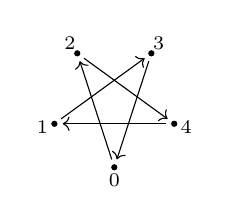
\begin{tikzpicture}[baseline=(b.base),scale=.8,every edge/.append style = {shorten <=3,shorten >=3}]
    \coordinate (b) at (0,0);
    \foreach \i in {0,...,4} {
      \filldraw ({(\i+3/4)*360/5}:1) circle (.04);
      \draw ({((-\i+3)+3/4)*360/5}:1.2) node {$\scriptstyle\i$};
      \draw[shorten <=2,shorten >=2] ({(\i+3/4)*360/5}:1) edge[<-] ({(\i+2+3/4)*360/5}:1);
    }
    % \draw (0,-1.6) node {$m=5$};
  \end{tikzpicture}
  \qquad\qquad\qquad\qquad
  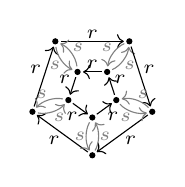
\begin{tikzpicture}[baseline=(b.base),scale=.8,every edge/.append style = {shorten <=2,shorten >=2}]
    \coordinate (b) at (0,0);
    \foreach \i in {0,...,4} {
      \filldraw ({(\i+3/4)*360/5}:1) circle (.04);
      \filldraw ({(\i+3/4)*360/5}:.4) circle (.04);
      \draw ({(\i+3/4)*360/5}:1) edge[<-,inner sep=0.2ex,"$\scriptstyle r$"'] ({(\i+1+3/4)*360/5}:1);
      \draw ({(\i+3/4)*360/5}:.4) edge[->,inner sep=0.2ex,"$\scriptstyle r$"'] ({(\i+1+3/4)*360/5}:.4);
      \draw ({(\i+3/4)*360/5}:1) edge[->,bend right,gray,inner sep=0.1ex,"$\scriptstyle s$"'] ({(\i+3/4)*360/5}:.4);
      \draw ({(\i+3/4)*360/5}:.4) edge[->,bend right,gray,inner sep=0.1ex,"$\scriptstyle s$"'] ({(\i+3/4)*360/5}:1);
    }
  \end{tikzpicture}
\]
Our main result in this section is that this type satisfies the following
property. We recall that the delooping operation is functorial, see
\cref{delooping-functorial} and~\cite{warn2023eilenberg}: in particular, we can
deloop morphisms. We also recall that the \emph{kernel} of a map $f:A\to B$ with $B$ pointed is its fiber at the distinguished element $\pt{}$ of~$B$.


\begin{theorem}[\agda{Cayley}{Cayley-ker}]
  \label{flattening-cayley}
  The type $\Cayley XG$ is the kernel of the function $\B\freegroup \gamma:\B\freegroup X\to\B G$ induced by~$\gamma$, \ie we have
  \[
    \Cayley XG
    \qeq
    \Sigma(x:\B X^*).(\pt{}=\B\freegroup\gamma(x))
    \text.
  \]
\end{theorem}

\begin{proof}
  We define the type family $P:\B\freegroup X\to\U$ by
  $P(x)=(\pt{}=\B\freegroup \gamma(x))$. Remember that $\B\freegroup X$ admits a
  description as a coequalizer, see \cref{wedge-of-circles} and
  \cref{bouquet-loop-space}. Hence, by the flattening lemma for coequalizers
  (see \cref{flattening-coequalizers} and \cite[Section~6.12]{hottbook}), we
  have a coequalizer of total spaces
  \[
    \begin{tikzcd}
      \Sigma X.P(\pt{})
      \ar[r,shift left,"{(x,p)\mapsto(\pt{},p)}"]
      \ar[r,shift right,"{(x,p)\mapsto(\pt{},\subst Pp(x))}"']
      &[50]
      \Sigma 1.P(\pt{})
      \ar[r,dotted]
      &
      \Sigma \B\freegroup X.P
    \end{tikzcd}
  \]
  By using the properties of transport in path
  spaces~\cite[Theorem~2.11.3]{hottbook}, it can be shown that the bottom map
  sends $(x,p)$ to $(\pt{},p\pcomp\B\freegroup\gamma(x))$. Moreover,
  $\B\freegroup \gamma$ is pointed, so $P(\pt{})$ is equal to $\Loop\B G$,
  \ie $G$, and we have the following coequalizer:
  \[
    \begin{tikzcd}
      X\times G
      \ar[r,shift left,"{(x,g)\mapsto g}"]
      \ar[r,shift right,"{(x,g)\mapsto gx}"']
      &[20]
      G
      \ar[r,dotted]
      &
      \Sigma \B\freegroup X.P
    \end{tikzcd}
  \]
  If follows that $\Sigma\B\freegroup X.P$ consists in $\sizeof G$ points and a
  path $g=gx$ for each pair $(x,g):X\times G$, and is therefore equal to the
  Cayley graph $\Cayley XG$.
\end{proof}

\noindent
The above result can be interpreted as stating that we have a fiber sequence (see \cite[Section~8.4]{hottbook})
\[
  \begin{tikzcd}
    \Cayley XG\ar[r] & \B\freegroup X \ar[r]&\B G
  \end{tikzcd}
\]
which encodes the fact that we have an action of~$G$ on its Cayley graph, whose
homotopy quotient $\Cayley XG\hq G$ is $\B\freegroup X$,
see~\cite[Proposition~16]{lens}. Hence, we recover the canonical action of~$G$
on its Cayley graph.

\paragraph{Relations}
The long exact sequence of homotopy groups induced by the above fiber
sequence~\cite[Theorem 8.4.6]{hottbook} implies in particular that we have the
following short exact sequence of groups
\[
  \begin{tikzcd}
  \label{exseq-cayley}
    0\ar[r] &\Loop\Cayley XG\ar[r] &\freegroup X \ar[r]&G\ar[r] & 0
  \end{tikzcd}
\]
which shows that $\Loop\Cayley XG$ is the (free) group encoding relations of~$G$
with respect to~$X$. Indeed, we have that $\Cayley XG=\B\freegroup R$ where $R$
is a choice of $\sizeof G\times(\sizeof X-1)+1$ relations: those are the loops
in the Cayley graph after contracting $\sizeof G-1$ edges to obtain a wedge of
circles. In some sense, \cref{flattening-cayley} provides an internalization of
the fact that~$G$ is presented by $\pres XR$, contrasting with the point of view
developed in \cref{delooping-hit}.

\paragraph{The Cayley complex and higher variants}

\appendix
\section{Omitted proofs}
\label{omitted-proofs}
\begin{proof}[Proof of \cref{loop-PG}]
  % Note that any element $f:\Aut\P G$, \ie morphism of actions $f:\P G\to\P G$,
  % satisfies $xf(y)=f(xy)$ for any $x,y:G$.
  The two functions
  \begin{align*}
    \phi:\Aut\P G&\to G
    &
    \psi:G&\to\Aut\P G
    \\
    f&\mapsto f(1)
    &
    x&\mapsto y\mapsto yx
  \end{align*}
  % $\phi:\Aut\P G\to G$ and $\psi:G\to\Aut\P G$, respectively defined by
  % $\phi(f)\defd f(1)$ and $\psi(x)(y)\defd yx$
  are group morphisms. Namely, given $f,g:\Aut\P G$, we have
  \begin{align*}
    \phi(g\circ f)&=g\circ f(1)=g(f(1)1)=f(1)g(1)=\phi(f)\phi(g)
    &
    \phi(\id)&=\id(1)=1
  \end{align*}
  and given $x,y:G$, we have for every $z:G$,
  \begin{align*}
    \psi(xy)(z)&=z(xy)=(zx)y=\psi(y)\circ\psi(x)(z)
    &
    \psi(1)(x)&=x1=\id(x)
  \end{align*}
  Moreover, they are mutually inverse. Namely, given $f:\Aut\P G$ and $x:G$, we
  have
  \begin{align*}
    \psi\circ\phi(f)(x)&=xf(1)=f(x1)=f(x)
    &
    \phi\circ\psi(x)&=1x=x    
  \end{align*}
  We thus have $\Aut\P G\simeq G$ and we conclude by univalence.
\end{proof}

\begin{proof}[Proof of \cref{fiberwise-embedding}]
  By definition, the map $\Sigma A.f$ is an embedding iff for every $(a,x)$ and
  $(a',x')$ in $\Sigma A X$, the induced map
  \[
    (a, x) = (a', x') \to (a, f\,a\,x) = (a', f\,a'\,x')
  \]
  is an equivalence. By the characterization of equalities in
  $\Sigma$-types~\cite[Theorem~2.7.2]{hottbook}, this map corresponds to a map
  \[
    (\Sigma(p : a = a').\subst Pp(x) = x') \to (\Sigma(p : a = a').\subst Qp(f\,a\,x) = f\,a'\,x')
  \]
  By \cite[Theorem~4.7.7]{hottbook}, this is an equivalence if and only if the
  fiber map
  \[
    (\subst Pp(x) = x') \to (\subst Qp(f\,a\,x) = f\,a'\,x')
  \]
  is an equivalence for every $p : a = a'$. By path induction, this is true if
  and only if
  \[
    \ap{(f\,a)} : x = x' \to f\,a\,x = f\,a\,x'
  \]
  is an equivalence for all $a : A$, and $x,x' : X a$. By definition, this is
  the requirement that $f\,a$ is an embedding for all $a : A$.
\end{proof}

\section{Equivalence between internal and external groups}
\paragraph{Functoriality of delooping}
\label{delooping-functorial}
One of the main properties of the delooping operation is that it is a ``local
inverse'' to taking loop spaces in the following sense:

\begin{proposition}
  \label{delooping-morphisms}
  Given pointed connected groupoids $A$ and~$B$ and a group morphism
  $f:\Loop A\to\Loop B$, there is a unique pointed morphism $g:A\to B$ such
  that $\Loop g=f$.
\end{proposition}
\begin{proof}
  By~\cite[Corollary~12]{warn2023eilenberg}, with $n=0$, we have that the type
  $\Sigma(g:A\to B).\Loop g=f$ is equivalent to
  $(p,q:\pt{A}=\pt{A})\to f(p\pcomp q)=f(p)\pcomp f(q)$. This type is a
  proposition because $\Loop B$ is a set (because $B$ is a groupoid), and
  inhabited (because $f$ is a morphism of groups), and thus contractible.
\end{proof}

\noindent
As an immediate consequence of the above lemma, deloopings are unique:

\begin{proposition}
  \label{delooping-unique}
  Given two deloopings $\B G$ and $\B' G$ of a group~$G$, we have $\B G=\B' G$.
\end{proposition}

\noindent
Given a group morphism $f:G\to H$ such that both~$G$ and~$H$ admit deloopings
(and this actually always holds by \cref{PG-delooping}), the \emph{delooping} of~$f$ is the morphism
\[
  \B f:\B G\to\B H
\]
associated, by \cref{delooping-morphisms}, to the morphism
$\transportinv{\Beq H}\circ f\circ\transport{\Beq G}:\Loop\B G\to\Loop\B
H$. By \cref{delooping-morphisms}, this operation is functorial in the sense
that that it preserves identities and composition.

\paragraph{Equivalence between the two points of view}
Although this is not central in this article, we shall mention here the
fundamental equivalence provided by the above constructions; details can be
found in~\cite{symmetry}.
%
We write $\IGroup$ for the type of internal groups, \ie pointed connected
groupoids.

% fact that the functions $\Loop$ and $\B$ defined above actually induce an
% equivalence between pointed connected groupoids and groups.

\begin{theorem}
  \label{internal-external-equivalence}
  The maps $\Loop:\IGroup\to\Group$ and $\B:\Group\to\IGroup$ form an
  equivalence of types.
\end{theorem}
\begin{proof}
  Given a group~$G$, we have $\Loop\B G=G$ by definition of~$\B G$. Given an
  internal group~$A$, we have $\B\Loop A\simeq A$ by \cref{delooping-unique}.
\end{proof}

\noindent
The above theorem thus states looping and delooping operators allow us to go
back and forth between the external and the internal point of view of group
theory in homotopy type theory. Note that the torsor construction only gives a
delooping in a larger universe than the original group unless one makes
additional assumptions such as the \emph{replacement
  axiom}~\cite[Axiom~18.1.8]{rijke2022introduction}.

% \noindent
% More generally, it is expected that the types $\IGroup[n]$ of pointed connected
% $n$-types provide a reasonable notion of ``higher-dimensional groups''.

\paragraph{Internal group actions}
In a similar way that the traditional notion of group admits an internal
reformulation (\cref{internal-groups}), the notion of action also admits an
internal counterpart which can be defined as follows.
%
Given a group~$G$, an \emph{internal} action of $G$ on a set $A$ is a function
\[
  \alpha : \B G \to \Set
\]
such that $\alpha(\pt{})=A$. Since $\Set$ is a
groupoid~\cite[Theorem 7.1.11]{hottbook}, by
\cref{internal-external-equivalence}, we have equivalences of types
\[
  (\B G\to\Set)
  \quad\equivto\quad
  (\Loop\B G\to\Loop(\Set,A))
  \quad\equivto\quad
  (G\to\Aut A)
\]
which show that internal group actions correspond to external ones: the
delooping operator internalizes an external group action, and the looping
operator externalizes an internal group action.
% \EO{faire le même schema pour les groupes internes et externes avec $\B$ et
% $\Loop$ d'un coté et de l'autre}


% BEGIN unchanged author comp.tex
\section{Connected components}
\label{connected-component}
We define the \emph{connected component} of the pointed type~$A$ as the type of
points which are merely connected to the distinguished point of~$A$. This type
is noted~$\Comp A$ (or $\Comp(A,\pt{})$ when we want to specify the
distinguished element~$\pt{}$). Formally,
\[
  \Comp A
  \qdefd
  \Sigma(x:A).\ptrunc{\pt{}=x}
\]
This type is canonically pointed by $(\pt{},\ptrunq{\refl{}})$.
%
This construction deserves its name because it produces a connected space, whose
geometry is the same as the original space around the distinguished point, as
shown in the following two lemmas.

\begin{lemma}[\agda{Comp}{isConnectedComp}]
  The type $\Comp A$ is connected.
\end{lemma}
\begin{proof}
  It can be shown that a type~$X$ is connected precisely when both $\ptrunc{X}$
  and $(x,y:X)\to\ptrunc{x=y}$ are inhabited, \ie when~$X$ merely has a point
  and any two points are merely equal~\cite[Exercise~7.6]{hottbook}.
  %
  In our case, the type $\Comp A$ is pointed and thus $\ptrunc{\Comp A}$
  holds.
  %
  Moreover, suppose that there are two points $(x,p)$ and $(y,q)$ in $\Comp A$
  with $x,y:A$, $p:\ptrunc{\pt{}=x}$ and $q:\ptrunc{\pt{}=y}$. Our goal is to
  show that $\ptrunc{(x,p)=(y,q)}$ holds, which is a proposition, so by
  elimination of propositional truncation, we can therefore assume that $p$
  (\resp $q$) has type $\pt{}=x$ (\resp $\pt{}=y$). Hence, we can construct a path
  $\sym p\pcomp q$ of type $x=y$, and therefore $(x,p)=(y,q)$ because the second
  components belong to a proposition by propositional truncation. We conclude
  that $\ptrunc{(x,p)=(y,q)}$ and finally that $\Comp A$ is connected.
\end{proof}

\begin{lemma}[\agda{Comp}{loopCompIsLoop}]
  \label{loop-comp}
  We have $\Loop\Comp A=\Loop A$.
\end{lemma}
\begin{proof}
  % we want to encode *=x in Comp A as B x = (*=x) and therefore it is enough to
  % show that Sigma A.B is contractible
  We begin by showing that the type
  \begin{equation}
    \label{eq:loop-comp-contr}
    \Sigma((x,t):\Comp A).(\pt{}=x)
  \end{equation}
  is contractible. In order to do so, observe that we have the following
  equivalence of types:
  \begin{align*}
    \Sigma((x,t):\Comp A).(\pt{}=x)
    &\simeq
    \Sigma((x,t):\Sigma(x:A).\ptrunc{\pt{}=x}).(\pt{}=x)
    \\
    &\equivto
    \Sigma(x:A).(\ptrunc{\pt{}=x})\times(\pt{}=x)
    \\
    &\equivto
    \Sigma((x,p):\Sigma(x:A).(\pt{}=x)).\ptrunc{\pt{}=x}
  \end{align*}
  using classical associativity and commutativity properties of
  $\Sigma$-types. Moreover, the type $\Sigma(x:A).(\pt{}=x)$ is
  contractible~\cite[Lemma~3.11.8]{hottbook}, therefore the whole type on the
  last line is a proposition (as a sum of propositions over a proposition), and
  therefore also the original type \cref{eq:loop-comp-contr}. We write $\pt{}'$
  for the element $(\pt{},\ptrunc{\refl{\pt{}}})$ of $\Comp A$. The type
  \cref{eq:loop-comp-contr} is pointed by the canonical element
  $(\pt{}',\refl{})$ and thus contractible as a pointed proposition.

  We have a morphism
  \[
    \begin{array}{r@{\ }c@{\ }c@{\ }c@{\ }c@{\ }l}
      F:&((x,t):\Comp A)&\to&(\pt{}'=(x,t))&\to&(\pt{}=x)\\
      &(x,t)&&p&\mapsto&\cong\fst(p)
    \end{array}
  \]
  sending a path~$p$ to the path obtained by applying the first projection. It
  canonically induces a morphism
  \begin{align*}
    \Sigma((x,t):\Comp A).(\pt{}'=(x,t))&\to\Sigma((x,t):\Comp A).(\pt{}=x)\\
    ((x,t),p)&\mapsto((x,t),\cong\fst(p))
  \end{align*}
  between the corresponding total spaces. Since the left member is contractible
  (by~\cite[Lemma~3.11.8]{hottbook} again) and the right member is contractible
  (as shown above), this is an equivalence. By~\cite[Theorem~4.7.7]{hottbook},
  for every $x:\Comp A$, the fiber morphism $F x$ is also an equivalence. In
  particular, with $x$ being $\pt{}'$, we obtain $\Loop\Comp A\simeq\Loop A$ (as
  a type) and we can conclude by univalence. Note that the equivalence preserves
  the group structure so that the equality also holds in groups.
\end{proof}

\noindent
As a direct corollary of the two above lemmas, we have:

\begin{proposition}
  \label{B-loop}
  Given a pointed groupoid~$A$, $\Comp A$ is a delooping of~$\Loop A$.
\end{proposition}

\begin{remark}
  Some people write $\Aut A$ for $\Loop A$ and the above proposition states that
  we have $\B\Aut A=\Comp A$. For this reason, the (confusing) notation
  $\operatorname{BAut}A$ is also found in the literature for $\Comp A$.
\end{remark}

% Local Variables:
% TeX-master: "article"
% End:

% END unchanged author comp.tex


\section{The flattening lemma}
We recall here the classical flattening lemma, see \cite[Section~6.12]{hottbook}
for a more detailed presentation and proof.

\begin{lemma}[Flattening for coequalizers]
  \label{flattening-coequalizers}
  Suppose given a coequalizer
  \[
    \begin{tikzcd}
      A\ar[r,shift left,"f"]\ar[r,shift right,"g"']&B\ar[r,dotted,"h"]&C
    \end{tikzcd}
  \]
  with $p:h\circ f=h\circ g$, and a type family $P:C\to\U$. Then the diagram
  \[
    \begin{tikzcd}[sep=huge]
      \Sigma A.(P\circ h\circ f)\ar[r,shift left,"\Sigma f.(\lambda\_.\id{})"]\ar[r,shift right,"\Sigma g.e"']&\Sigma B.(P\circ h)\ar[r,dotted,"\Sigma h.(\lambda\_.\id{})"]&\Sigma C.P
    \end{tikzcd}
  \]
  is a coequalizer, where the map
  \[
    e:(a:A)\to P(h(f(a)))\to P(h(g(a)))
  \]
  is induced by transport along~$p$ by
  \[
    e\,a\,x\defd
    \subst{P}{\happly pa}(x)
    \text.
  \]
\end{lemma}

\noindent
Note that there is a slight asymmetry: we could have formulated a similar
statement with $\Sigma A.(P\circ h\circ g)$ as left object.

% \section{Rijke's proof}
% \input{rijke}

% Local Variables:
% TeX-master: "article"
% End:

\begin{thebibliography}{10}

\bibitem{polygraphs}
Dimitri Ara, Albert Burroni, Yves Guiraud, Philippe Malbos, François Métayer,
  and Samuel Mimram.
\newblock Polygraphs: From rewriting to higher categories.
\newblock To appear, 2023.
\newblock \href {https://arxiv.org/abs/2312.00429} {\path{arXiv:2312.00429}}.

\bibitem{symmetry}
Marc Bezem, Ulrik Buchholtz, Pierre Cagne, Bjørn~Ian Dundas, and Daniel~R.
  Grayson.
\newblock Symmetry.
\newblock URL: \url{https://github.com/UniMath/SymmetryBook}.

\bibitem{bezem2021construction}
Marc Bezem, Ulrik Buchholtz, Daniel~R Grayson, and Michael Shulman.
\newblock Construction of the circle in {UniMath}.
\newblock {\em Journal of Pure and Applied Algebra}, 225(10):106687, 2021.
\newblock \href {https://arxiv.org/abs/1910.01856} {\path{arXiv:1910.01856}},
  \href {https://doi.org/10.1016/j.jpaa.2021.106687}
  {\path{doi:10.1016/j.jpaa.2021.106687}}.

\bibitem{brunerie2022synthetic}
Guillaume Brunerie, Axel Ljungstr{\"o}m, and Anders M{\"o}rtberg.
\newblock Synthetic integral cohomology in cubical {A}gda.
\newblock In {\em 30th EACSL Annual Conference on Computer Science Logic (CSL
  2022)}. Schloss Dagstuhl-Leibniz-Zentrum f{\"u}r Informatik, 2022.
\newblock \href {https://doi.org/10.4230/LIPIcs.CSL.2022.11}
  {\path{doi:10.4230/LIPIcs.CSL.2022.11}}.

\bibitem{buchholtz2023central}
Ulrik Buchholtz, J~Daniel Christensen, Jarl G~Taxer{\aa}s Flaten, and Egbert
  Rijke.
\newblock Central {H}-spaces and banded types.
\newblock Preprint, 2023.
\newblock \href {https://arxiv.org/abs/2301.02636} {\path{arXiv:2301.02636}}.

\bibitem{buchholtz2020cellular}
Ulrik Buchholtz and Kuen-Bang Hou.
\newblock Cellular cohomology in homotopy type theory.
\newblock {\em Logical Methods in Computer Science}, 16, 2020.
\newblock \href {https://arxiv.org/abs/1802.02191} {\path{arXiv:1802.02191}},
  \href {https://doi.org/10.23638/LMCS-16(2:7)2020}
  {\path{doi:10.23638/LMCS-16(2:7)2020}}.

\bibitem{buchholtz2017real}
Ulrik Buchholtz and Egbert Rijke.
\newblock The real projective spaces in homotopy type theory.
\newblock In {\em 2017 32nd Annual ACM/IEEE Symposium on Logic in Computer
  Science (LICS)}, pages 1--8. IEEE, 2017.
\newblock \href {https://arxiv.org/abs/1704.05770} {\path{arXiv:1704.05770}},
  \href {https://doi.org/10.5555/3329995.3330081}
  {\path{doi:10.5555/3329995.3330081}}.

\bibitem{cavallo2015synthetic}
Evan Cavallo.
\newblock {\em Synthetic cohomology in homotopy type theory}.
\newblock PhD thesis, MA thesis, 2015.

\bibitem{cayley1878desiderata}
Arthur Cayley.
\newblock Desiderata and suggestions. {N}o. 2 -- {T}he theory of groups:
  graphical representation.
\newblock {\em American journal of mathematics}, 1(2):174--176, 1878.

\bibitem{git}
Camil Champin and Samuel Mimram.
\newblock Delooping generated groups.
\newblock URL: \url{https://github.com/smimram/generated-deloopings-agda}.

\bibitem{coquand2013isomorphism}
Thierry Coquand and Nils~Anders Danielsson.
\newblock Isomorphism is equality.
\newblock {\em Indagationes Mathematicae}, 24(4):1105--1120, 2013.
\newblock \href {https://doi.org/10.1016/j.indag.2013.09.002}
  {\path{doi:10.1016/j.indag.2013.09.002}}.

\bibitem{demazure1970groupes}
Michel Demazure and Pierre Gabriel.
\newblock {\em Groupes Alg{\'e}briques, Tome 1}.
\newblock North-Holland Publishing Company, 1970.

\bibitem{groves2006rewriting}
John~RJ Groves.
\newblock Rewriting systems and homology of groups.
\newblock In {\em Groups—Canberra 1989: Australian National University Group
  Theory Program 1989}, pages 114--141. Springer, 2006.
\newblock \href {https://doi.org/10.1007/BFb0100735}
  {\path{doi:10.1007/BFb0100735}}.

\bibitem{kapulkin2021simplicial}
Krzysztof Kapulkin and Peter~LeFanu Lumsdaine.
\newblock {The simplicial model of Univalent Foundations (after Voevodsky)}.
\newblock {\em Journal of the European Mathematical Society}, 23(6):2071--2126,
  2021.
\newblock \href {https://arxiv.org/abs/1211.2851} {\path{arXiv:1211.2851}},
  \href {https://doi.org/10.4171/jems/1050} {\path{doi:10.4171/jems/1050}}.

\bibitem{kraus2018free}
Nicolai Kraus and Thorsten Altenkirch.
\newblock Free higher groups in homotopy type theory.
\newblock In {\em Proceedings of the 33rd Annual ACM/IEEE Symposium on Logic in
  Computer Science}, pages 599--608, 2018.
\newblock \href {https://arxiv.org/abs/1805.02069} {\path{arXiv:1805.02069}},
  \href {https://doi.org/10.1145/3209108.3209183}
  {\path{doi:10.1145/3209108.3209183}}.

\bibitem{kraus2022rewriting}
Nicolai Kraus and Jakob von Raumer.
\newblock A rewriting coherence theorem with applications in homotopy type
  theory.
\newblock {\em Mathematical Structures in Computer Science}, 32(7):982--1014,
  2022.
\newblock \href {https://arxiv.org/abs/2107.01594} {\path{arXiv:2107.01594}},
  \href {https://doi.org/10.1017/S0960129523000026}
  {\path{doi:10.1017/S0960129523000026}}.

\bibitem{licata2014eilenberg}
Daniel~R Licata and Eric Finster.
\newblock {Eilenberg-MacLane spaces in homotopy type theory}.
\newblock In {\em Proceedings of the Joint Meeting of the Twenty-Third EACSL
  Annual Conference on Computer Science Logic (CSL) and the Twenty-Ninth Annual
  ACM/IEEE Symposium on Logic in Computer Science (LICS)}, pages 1--9, 2014.
\newblock \href {https://doi.org/10.1145/2603088.2603153}
  {\path{doi:10.1145/2603088.2603153}}.

\bibitem{lumsdaine2020semantics}
Peter~LeFanu Lumsdaine and Michael Shulman.
\newblock Semantics of higher inductive types.
\newblock {\em Mathematical Proceedings of the Cambridge Philosophical
  Society}, 169(1):159--208, 2020.
\newblock \href {https://arxiv.org/abs/1705.07088} {\path{arXiv:1705.07088}},
  \href {https://doi.org/10.1017/S030500411900015X}
  {\path{doi:10.1017/S030500411900015X}}.

\bibitem{lyndon1977combinatorial}
Roger~C Lyndon and Paul~E Schupp.
\newblock {\em Combinatorial group theory}, volume 188.
\newblock Springer, 1977.

\bibitem{martin1984intuitionistic}
Per Martin-L{\"o}f.
\newblock {\em Intuitionistic type theory}, volume~1 of {\em Studies in proof
  theory}.
\newblock Bibliopolis, 1984.

\bibitem{lens}
\'Emile Oleon and Samuel Mimram.
\newblock {Delooping cyclic groups with lens spaces in homotopy type theory}.
\newblock Accepted at LICS 2024 conference, 2024.

\bibitem{poincare1895analysis}
Henri Poincar{\'e}.
\newblock {\em Analysis situs}.
\newblock Gauthier-Villars Paris, France, 1895.

\bibitem{rijke2017join}
Egbert Rijke.
\newblock The join construction.
\newblock Preprint, 2017.
\newblock \href {https://arxiv.org/abs/1701.07538} {\path{arXiv:1701.07538}}.

\bibitem{rijke2018classifying}
Egbert Rijke.
\newblock {\em Classifying Types}.
\newblock PhD thesis, Carnegie Mellon University, July 2018.
\newblock \href {https://arxiv.org/abs/1906.09435} {\path{arXiv:1906.09435}}.

\bibitem{rijke2022introduction}
Egbert Rijke.
\newblock Introduction to homotopy type theory.
\newblock Preprint, 2022.
\newblock \href {https://arxiv.org/abs/2212.11082} {\path{arXiv:2212.11082}}.

\bibitem{cubicalagda}
{The Agda Community}.
\newblock {Cubical Agda Library}, July 2023.
\newblock URL: \url{https://github.com/agda/cubical}.

\bibitem{hottbook}
The {Univalent Foundations Program}.
\newblock {\em Homotopy Type Theory: Univalent Foundations of Mathematics}.
\newblock Institute for Advanced Study, 2013.
\newblock URL: \url{https://homotopytypetheory.org/book/}.

\bibitem{vezzosi2021cubical}
Andrea Vezzosi, Anders M{\"o}rtberg, and Andreas Abel.
\newblock {Cubical Agda: A dependently typed programming language with
  univalence and higher inductive types}.
\newblock {\em Journal of Functional Programming}, 31, 2021.
\newblock \href {https://doi.org/10.1145/3341691} {\path{doi:10.1145/3341691}}.

\bibitem{warn2023eilenberg}
David W{\"a}rn.
\newblock Eilenberg--maclane spaces and stabilisation in homotopy type theory.
\newblock {\em Journal of Homotopy and Related Structures}, 18(2):357--368,
  2023.
\newblock \href {https://arxiv.org/abs/2301.03685} {\path{arXiv:2301.03685}},
  \href {https://doi.org/10.1007/s40062-023-00330-5}
  {\path{doi:10.1007/s40062-023-00330-5}}.

\bibitem{warn2023path}
David W{\"a}rn.
\newblock Path spaces of pushouts.
\newblock Preprint, 2023.
\newblock \href {https://arxiv.org/abs/2402.12339} {\path{arXiv:2402.12339}}.

\end{thebibliography}
\end{document}
